\section{手法概要}
動画からレスキュー犬の行動を推定するための手法の概要は以下の通りである.
\begin{itemize}
 \item 動画から一定フレームと対応する音声を取出し整形.
 \item LSTMなどの時系列情報を扱う手法により,データから特徴量を抽出.
 \item 単位データから犬行動を分類するよう学習し,分類.
\end{itemize}

\section{予備実験}
データセットに犬の一人称視点動画DogCentric Activity Dataset(DCAD)~\cite{yumi2014first}を用い,これを分類する予備実験を行った.これは犬の散歩を記録したデータであり,災害救助活動やその訓練データではない.災害救助活動および訓練データは現在作成中である.
DCADデータセットは10クラス209クリップで構成されている.クラスはそれぞれ,横断前の待機\(Car\), 水分の摂取\(Drink\), 手渡しでの食事\(Feed\), 左を見る\(Look\_at\_Left\), 右を見る\(Look\_at\_Right\), 人間が犬を撫でる\(Pet\),ボールで遊ぶ\(Play\_with\_ball\), 体をブルブルと振る\(Shake\), 何かの臭いを嗅ぐ\(Sniff\), 歩く\(Walk\),である.

\begin{figure}[htbp]
%  \begin{center}
    \begin{tabular}{c}
     % 0
      \begin{minipage}{0.18\hsize}
        \begin{center}
          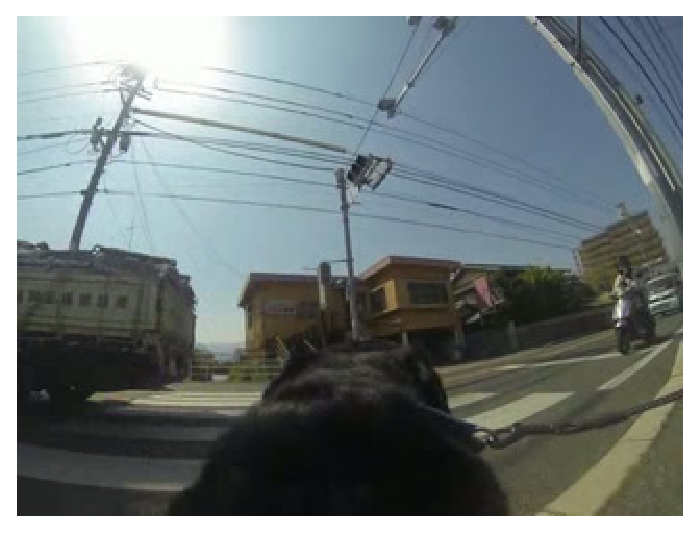
\includegraphics[clip, width=1.7cm]{./Img/HC005.eps}
          \hspace{0.3cm} { }
        \end{center}
      \end{minipage}
      \begin{minipage}{0.18\hsize}
        \begin{center}
          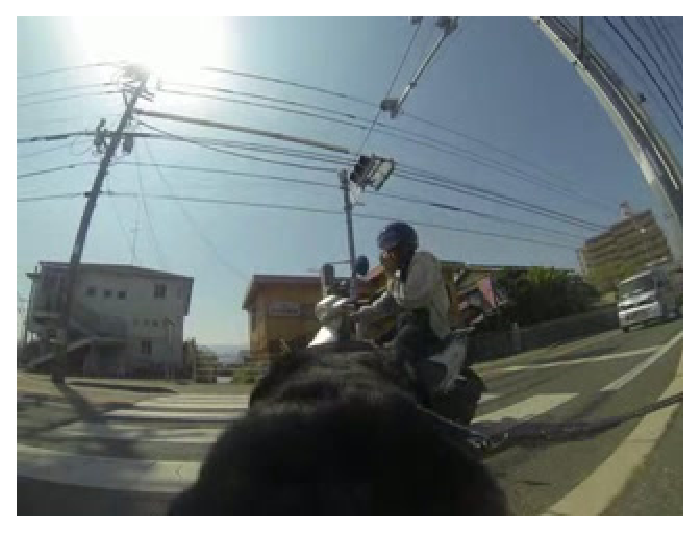
\includegraphics[clip, width=1.7cm]{./Img/HC006.eps}
          \hspace{0.3cm} { }
        \end{center}
      \end{minipage}

      % 2
      \begin{minipage}{0.18\hsize}
        \begin{center}
          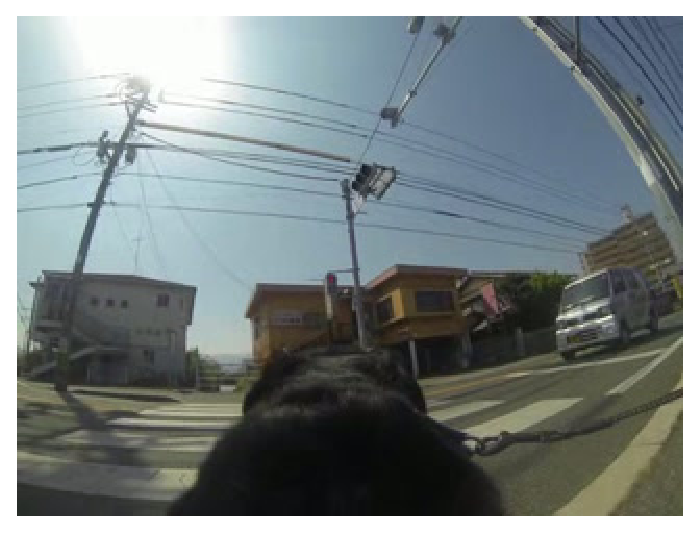
\includegraphics[clip, width=1.7cm]{./Img/HC007.eps}
          \hspace{0.0cm} {Car}
        \end{center}
      \end{minipage}

      % 4
      \begin{minipage}{0.18\hsize}
        \begin{center}
          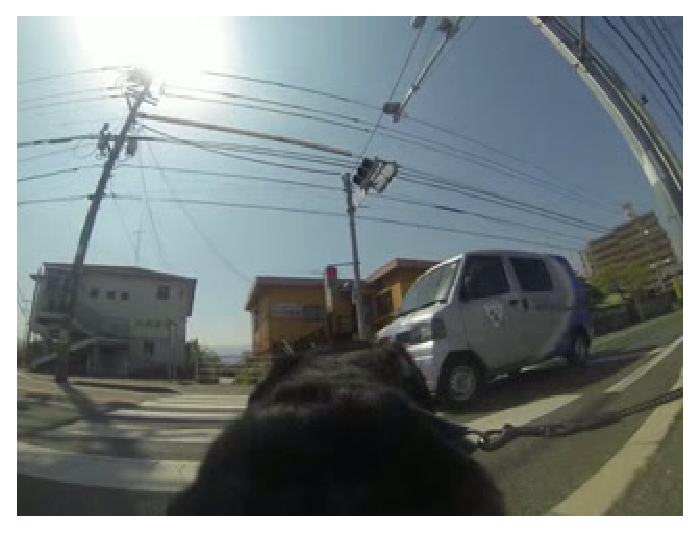
\includegraphics[clip, width=1.7cm]{./Img/HC008.eps}
          \hspace{0.1cm} { }
        \end{center}
      \end{minipage}
      % 5
      \begin{minipage}{0.18\hsize}
        \begin{center}
          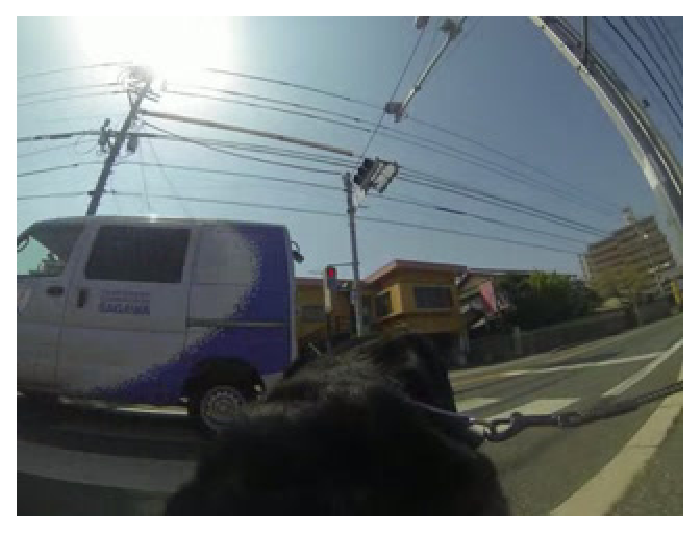
\includegraphics[clip, width=1.7cm]{./Img/HC009.eps}
          \hspace{0.2cm} { }
        \end{center}
      \end{minipage}
\\
     \begin{minipage}{0.18\hsize}
      \begin{center}
       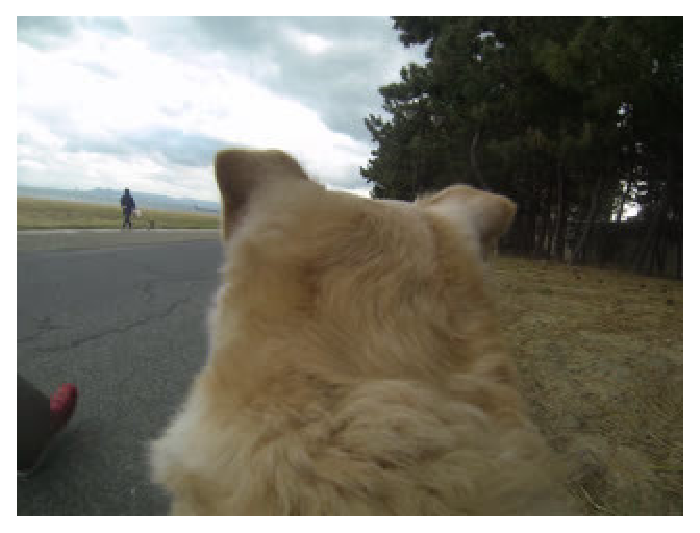
\includegraphics[clip, width=1.7cm]{./Img/KL001.eps}
       \hspace{0.3cm} { }
      \end{center}
     \end{minipage}
     \begin{minipage}{0.18\hsize}
      \begin{center}
       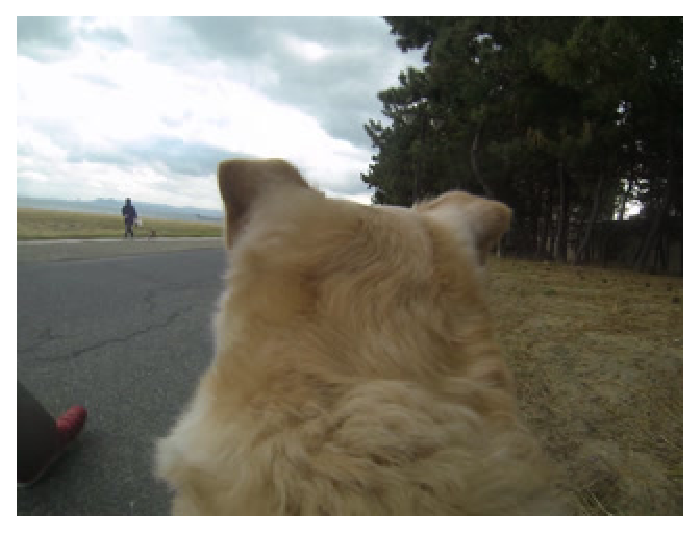
\includegraphics[clip, width=1.7cm]{./Img/KL002.eps}
       \hspace{0.3cm} { }
      \end{center}
     \end{minipage}
     \begin{minipage}{0.18\hsize}
      \begin{center}
       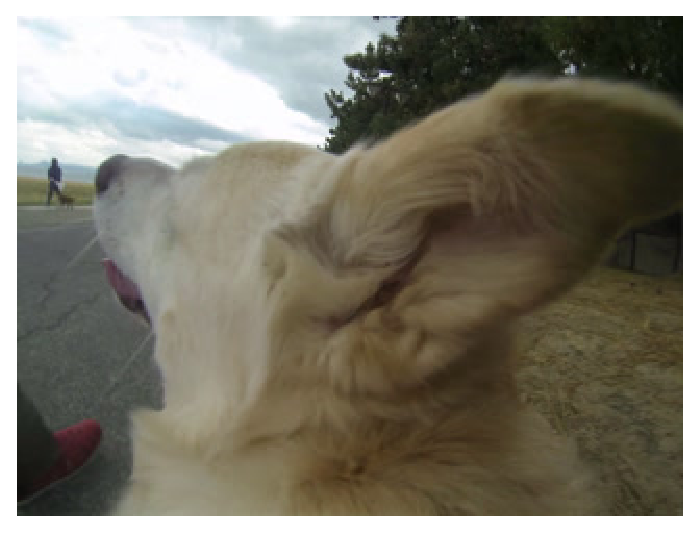
\includegraphics[clip, width=1.7cm]{./Img/KL003.eps}
       \hspace{0.1cm} {Look\_at\_Left} 
      \end{center}
     \end{minipage}
     \begin{minipage}{0.18\hsize}
      \begin{center}
       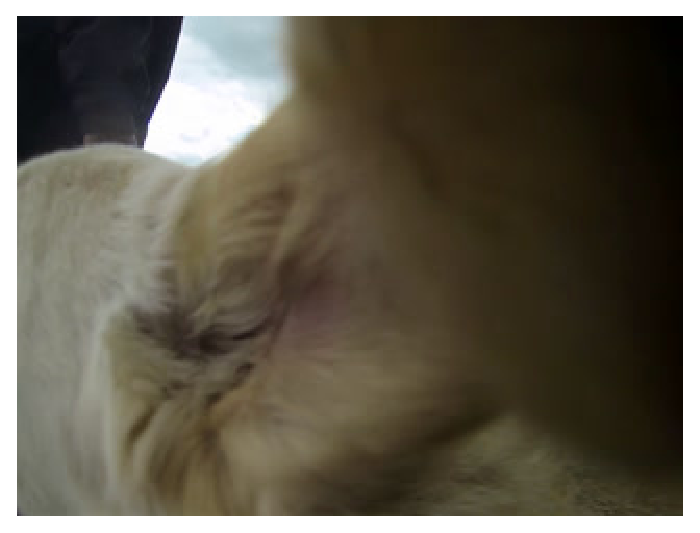
\includegraphics[clip, width=1.7cm]{./Img/KL004.eps}
       \hspace{1.3cm} { } 
      \end{center}
     \end{minipage}
     \begin{minipage}{0.18\hsize}
      \begin{center}
       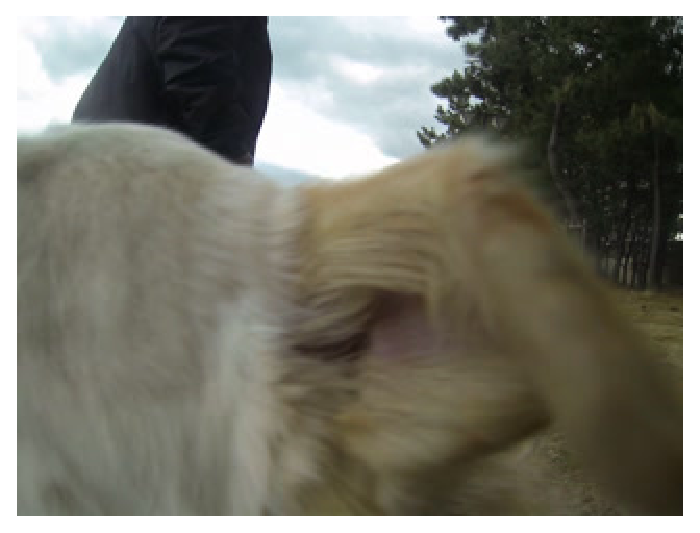
\includegraphics[clip, width=1.7cm]{./Img/KL005.eps}
       \hspace{1.6cm} { }
      \end{center}
     \end{minipage}

    \end{tabular}
    \caption{DogCentric Activity Dataset}
    \label{dcad_img}
%  \end{center}
\end{figure}

動画ひとつにつきフレーム全体の平均を取り~(式\ref{frame}\}),画像として扱い分類した~(図\ref{net}).ResNetとVGG16をそれぞれ用いたPre-trained modelのfine-tuningと二通り行った.

\begin{equation}
 \label{frame}
 Input = \frac{\Sigma^{sec \times FPS} Frame}{sec \times FPS}
\end{equation}

\begin{figure}[htbp]
 \begin{center}
  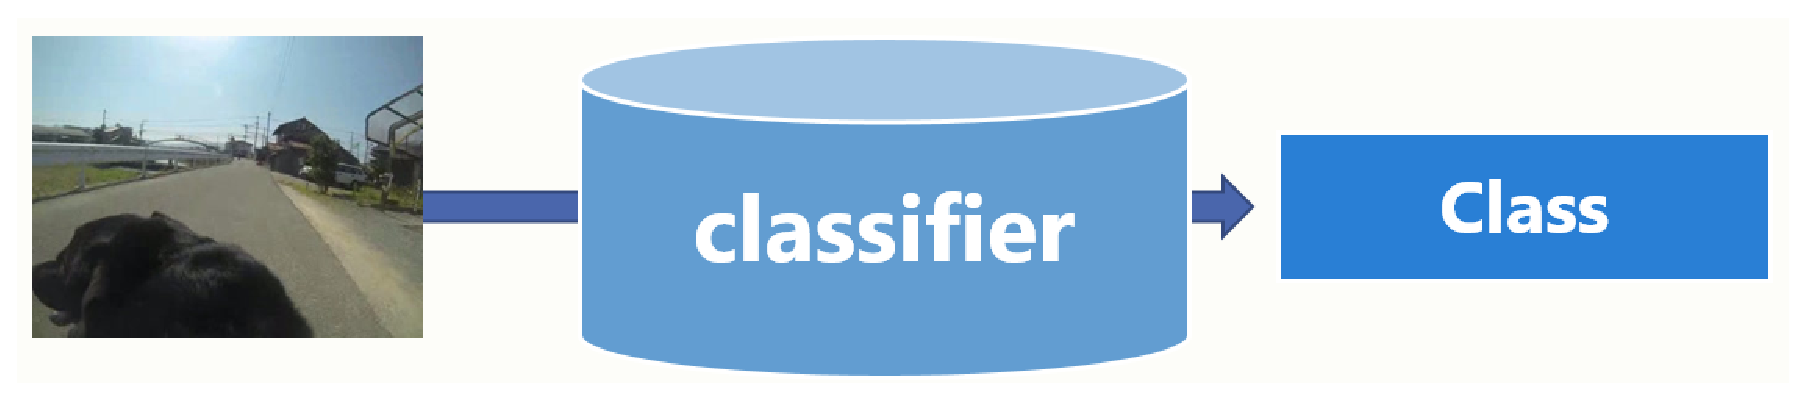
\includegraphics[width=8cm]{./Img/net.eps}
  \caption{ネットワーク}
  \label{net}
 \end{center}
\end{figure}

% \begin{figure}[htbp]
%  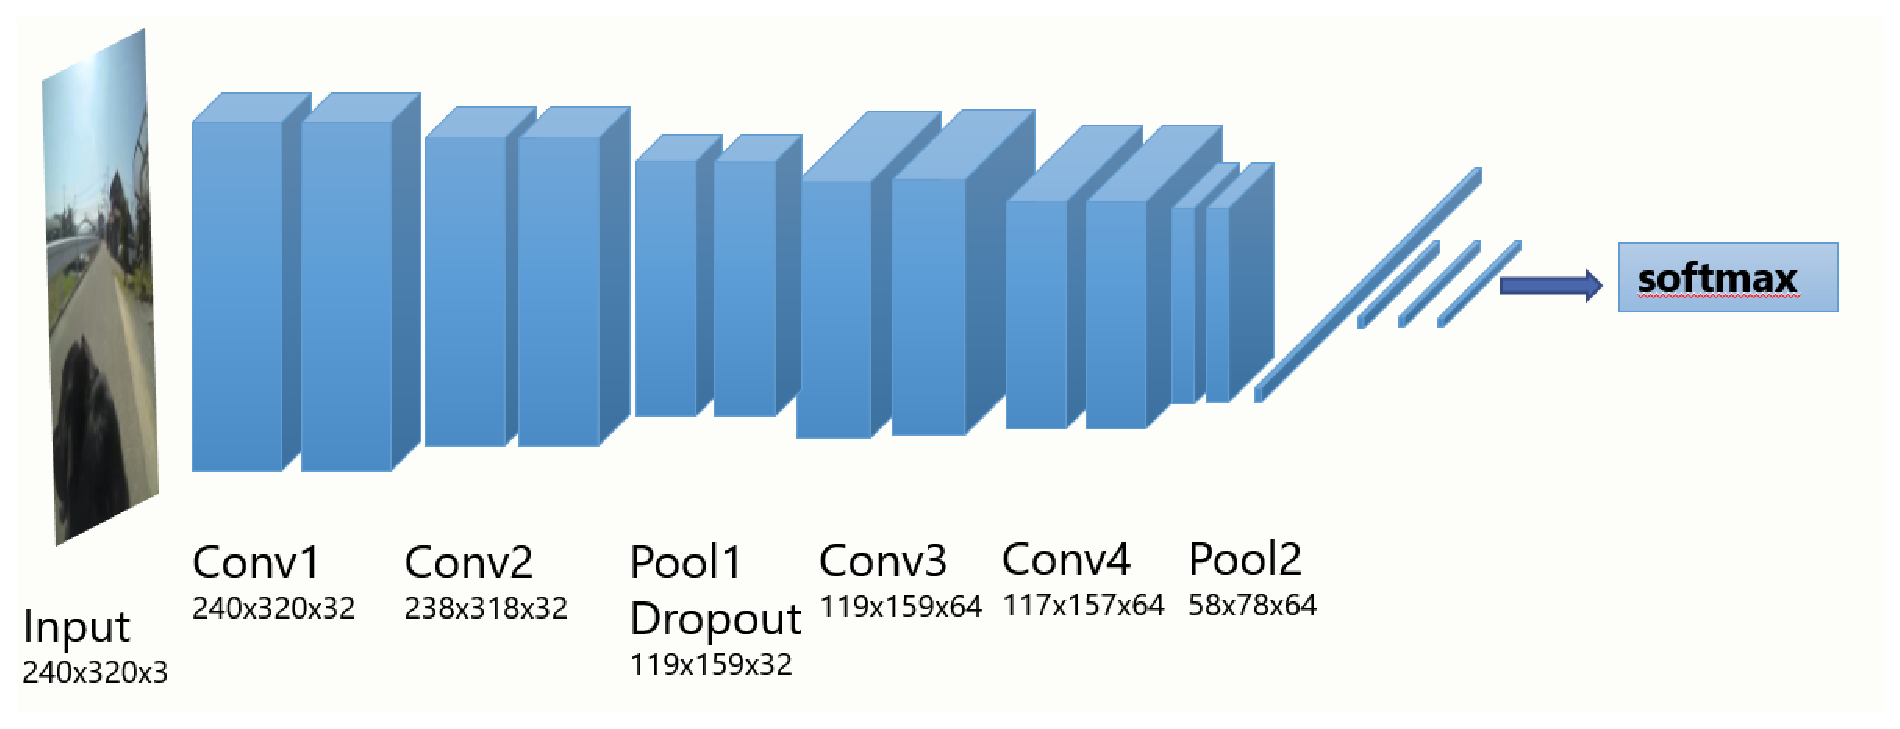
\includegraphics[width=10cm]{./Img/usemodel.eps}
%  \caption{利用したモデル}
%  \label{model}
% \end{figure}
% \begin{figure}[htbp]
%  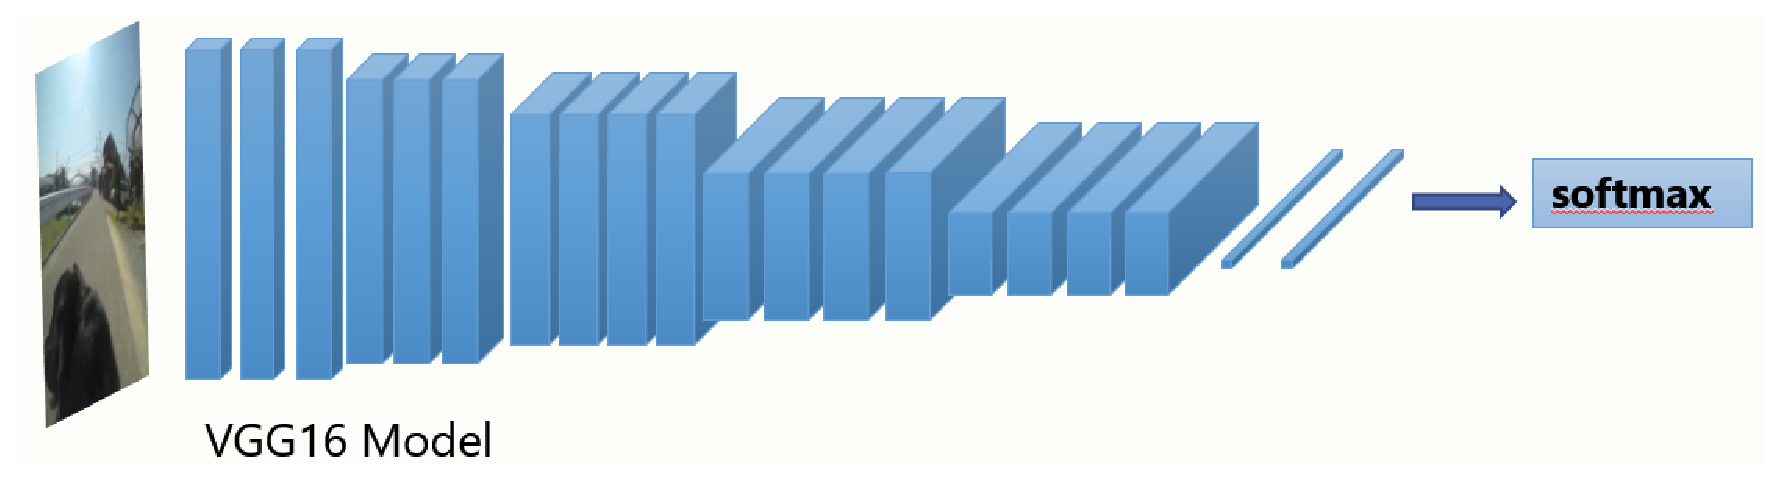
\includegraphics[width=8cm]{./Img/vgg16model.eps}
%  \caption{VGG16モデル}
%  \label{vgg16model}
% \end{figure}
\section{実験結果}
予備実験の結果を~(図\ref{vgg16_res},\ref{resnet_res})にそれぞれ示す.分類率は,VGG16モデルを利用したものが64.3\%,ResNetモデルを利用したものが59.5\%であった.
全般的に,データの多いクラスは精度が高い傾向にあるが,データの少ないクラスは精度が低い傾向にある.
加えて,~\(Car\)クラスは道路の進行方向に対して垂直に待機している10クラスの中で特殊なクラスであり,車などの写ったフレームの影響で分類精度が上昇していると考えられる.~\(Feed\)クラス,~\(Pet\)クラス,~\(Play\_with\_ball\)クラスは,それぞれフレーム内を人間が占める割合が多いクラスと言え,そのため混同が起こりやすいと考えられる.

%\(Look_at_Left\)クラスは


\begin{figure}[htbp]
 % \begin{tabular}{cc}
 %  \begin{minipage}{0.5\textwidth}
   \begin{center}
    
    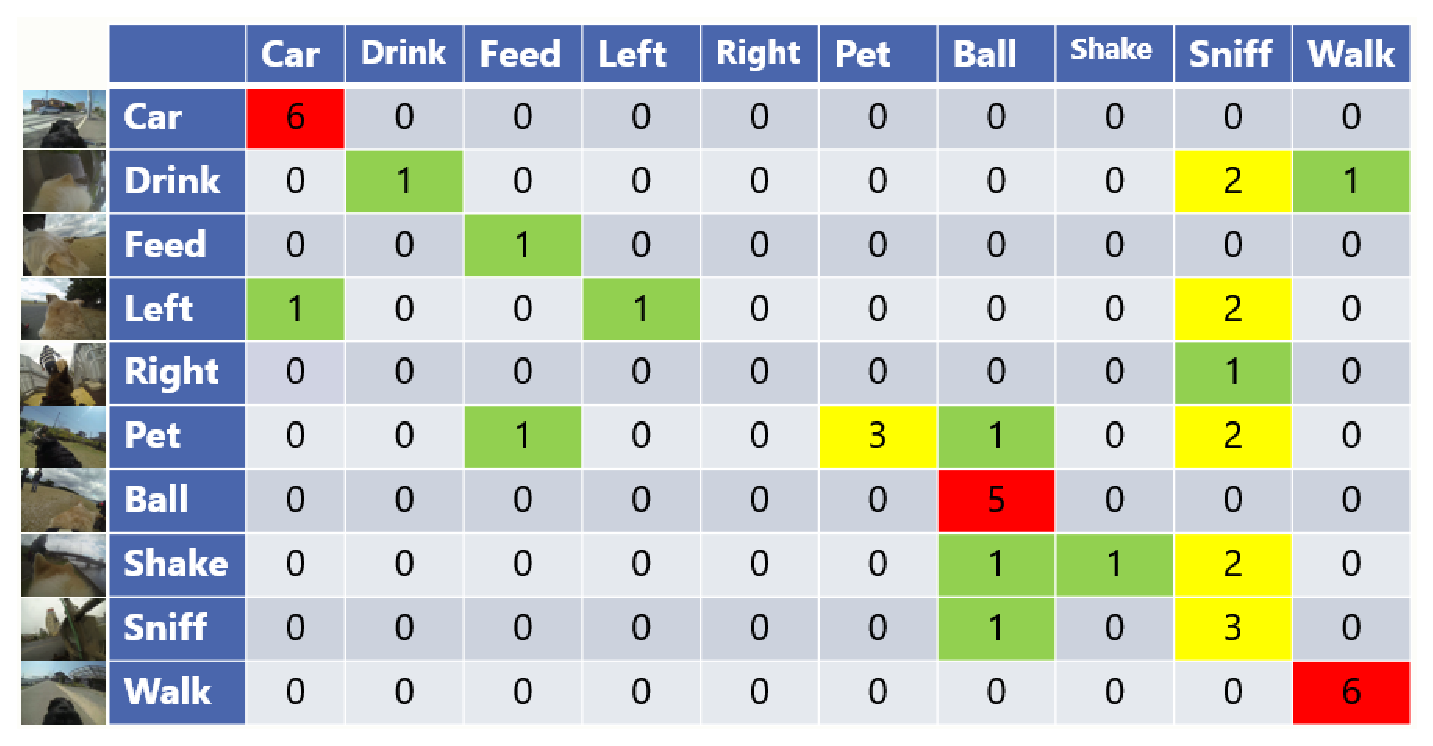
\includegraphics[scale=0.3]{./Img/vgg16_res.eps}
    \caption{VGG16 pretrained modelによるfinetuningの結果}
    \label{vgg16_res}
   \end{center}
  % \end{minipage}
  % \begin{minipage}{0.5\textwidth}
\end{figure}
\begin{figure}[htbp]

   \begin{center}

    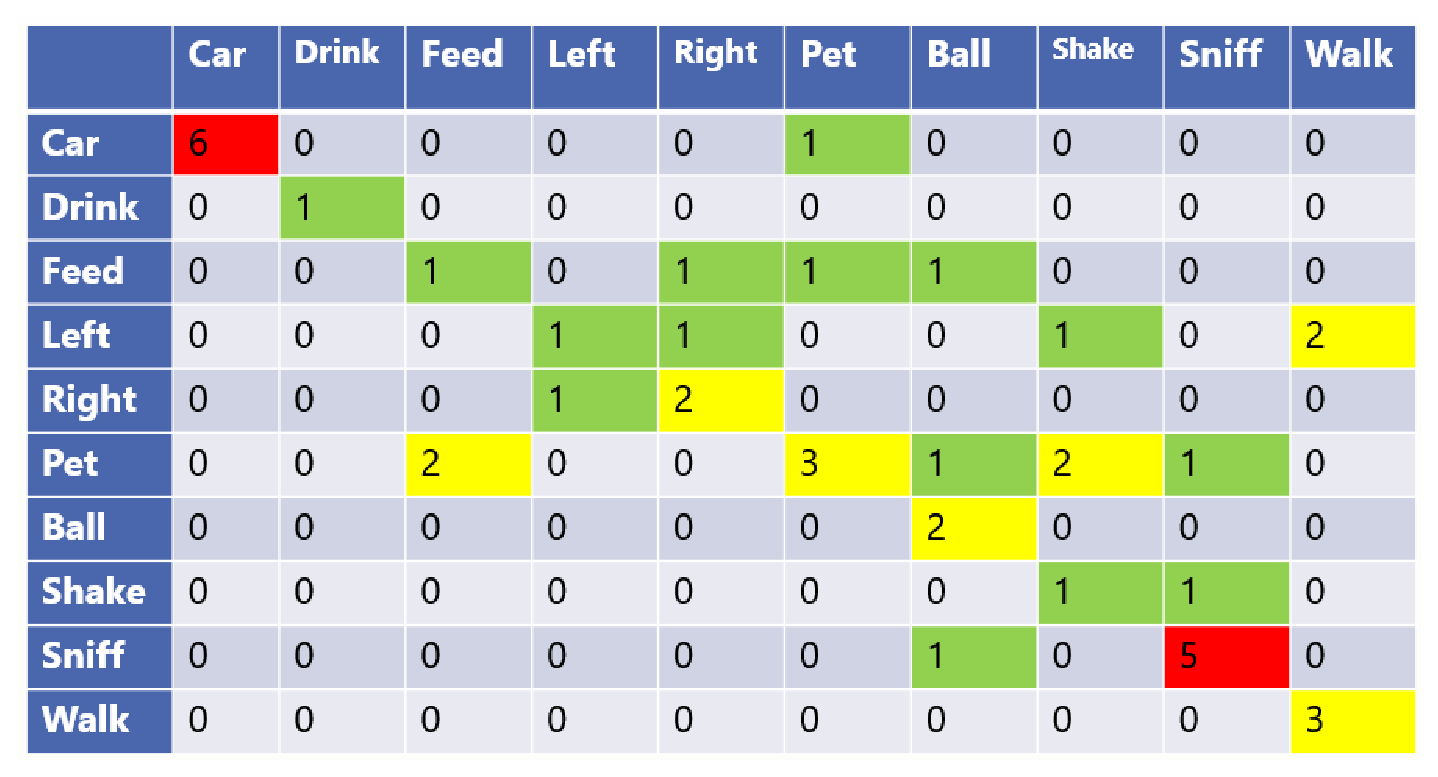
\includegraphics[scale=0.3]{./Img/resnet_res.eps}
  \caption{ResNet pretrained modelによるfinetuningの結果}
  \label{resnet_res}
   \end{center}
 %  \end{minipage}
 % \end{tabular}

\end{figure}

\section{まとめ,今後の課題}
動画の各フレームの平均を取り,画像として識別した.
データの少ないクラスは精度が低いため,データを補う必要がある.
予備実験では簡易的な方法を用いたが,今後は最新手法による分類を検討している.またレスキュー犬の行動を認識する際には複数クラスの出力にする必要がある.


今後の課題として,時系列情報を特徴量抽出に使う.
また,音声データから特徴量を抽出し,動画特徴量と併せたマルチモーダルな特徴量を利用し,レスキュー犬の行動分類を行う.


{\scriptsize % 7pt
%{\footnotesize % 8pt
%{\small % 9pt
%\bibliographystyle{ieee}
\bibliographystyle{junsrt}
\bibliography{ref}
}
% \begin{footnotesize}
% %{\small
% \bibliography{ref}
% \bibliographystyle{junsrt}
% %}
% \end{footnotesize}
\end{document}
